
\section{Getting started}\label{sect:start}\index{PISM!getting started}

In this section we give an extended example applying PISM to model the Greenland ice sheet.  We use recent data sets provided by the \href{http://websrv.cs.umt.edu/isis/index.php/SeaRISE_Assessment}{Sea-level Response to Ice Sheet Evolution (SeaRISE)} group.  SeaRISE is a community-organized assessment process providing an upper bound on ice sheet contributions to sea level in the next 100--200 years, especially for the next IPCC report in 2013.

The example in this section is a quick, hands-on first look at PISM.  It is not an in-depth tutorial, and some details of what is happening will only be explained later.  The sections on the older \mbox{EISMINT-Greenland} and \mbox{EISMINT-Ross} modeling cases, for instance, do a more complete job of explaining the ways users will need to preprocess not-so-clean input data and then make, and evaluate, modeling choices.

The PISM output figures in this section were produced using a supercomputer.  However, in order for the examples here to run on a typical workstation, a rather coarse $20\,\textrm{km}$ grid is used.  One purpose of PISM is to make much higher spatial resolution actually possible, but it does indeed require large-scale \emph{parallel} processing.


\subsection{Install PISM}

See the \emph{Installation Manual} at \href{http://www.pism-docs.org}{\texttt{www.pism-docs.org}}
to install PISM.  Once installed, executables \texttt{pismr} and \texttt{pclimate}, and several others, will be in the \texttt{bin} subdirectory of the main PISM directory.  The main PISM directory might be at \texttt{/home/username/pism-dev/}, for example.  The instructions below assume you start from that main PISM directory.  We also assume you are using a \texttt{bash} shell or at least one that accepts \texttt{bash} syntax.


\subsection{Obtain and preprocess the input data}

The NetCDF data file which we use for input is freely-available online.  Descriptions of the data it contains, and a link to the file itself, are on this web page: 
\medskip

\centerline{\protect{\textbf{\url{http://websrv.cs.umt.edu/isis/index.php/Present_Day_Greenland}}}}
\medskip

\noindent The quickest way to get the file is to do
\begin{verbatim}
$ cd examples/searise-greenland
$ ./preprocess.sh
\end{verbatim}
\noindent The script \texttt{preprocess.sh}\footnote{\protect{This script requires \texttt{wget} and also NCO (NetCDF Operators; \url{http://nco.sourceforge.net/})}.} downloads the version 1.1 SeaRISE ``master'' present-day data set and adjusts it to make it PISM-readable.  It creates three new NetCDF files, each having small metadata changes so that they can be read by PISM.  These metadata can be listed by \texttt{ncdump -h}.  Two of the new files contain famous time-dependent paleo-climate records from ice core (\texttt{pism_dT.nc} has GRIP) and seabed core records (\texttt{pism_dSL.nc} has SPECMAP).

Any of these NetCDF files can be viewed with \texttt{ncview} or other NetCDF visualization tools.  (See Table \ref{tab:NetCDFview} below.)  An application of IDV to the master data set produced Figure \ref{fig:sr-input}, for example.

\begin{figure}[ht]
\centering
\mbox{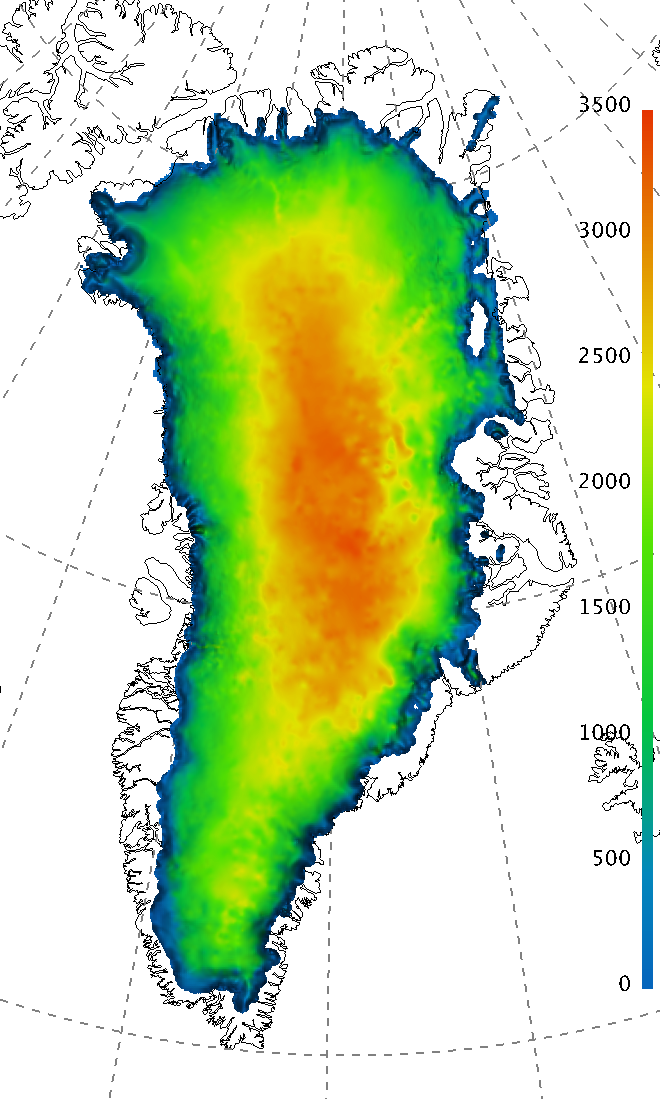
\includegraphics[width=2.0in,keepaspectratio=true]{sr-greenland-thk}
  \qquad
  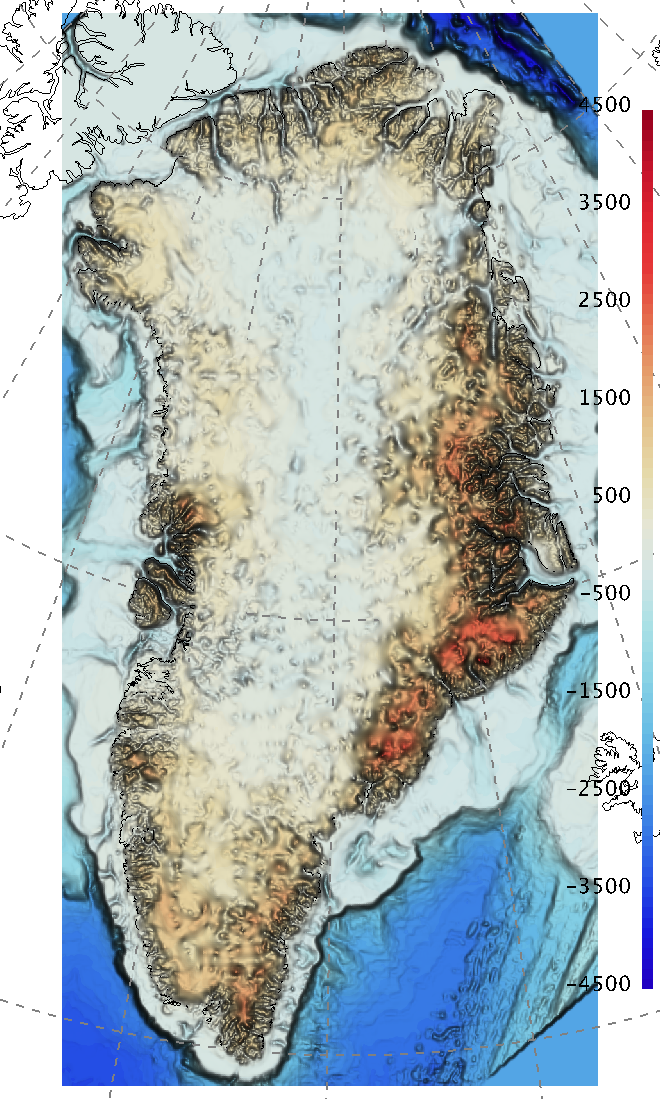
\includegraphics[width=2.0in,keepaspectratio=true]{sr-greenland-topg}
  \qquad
  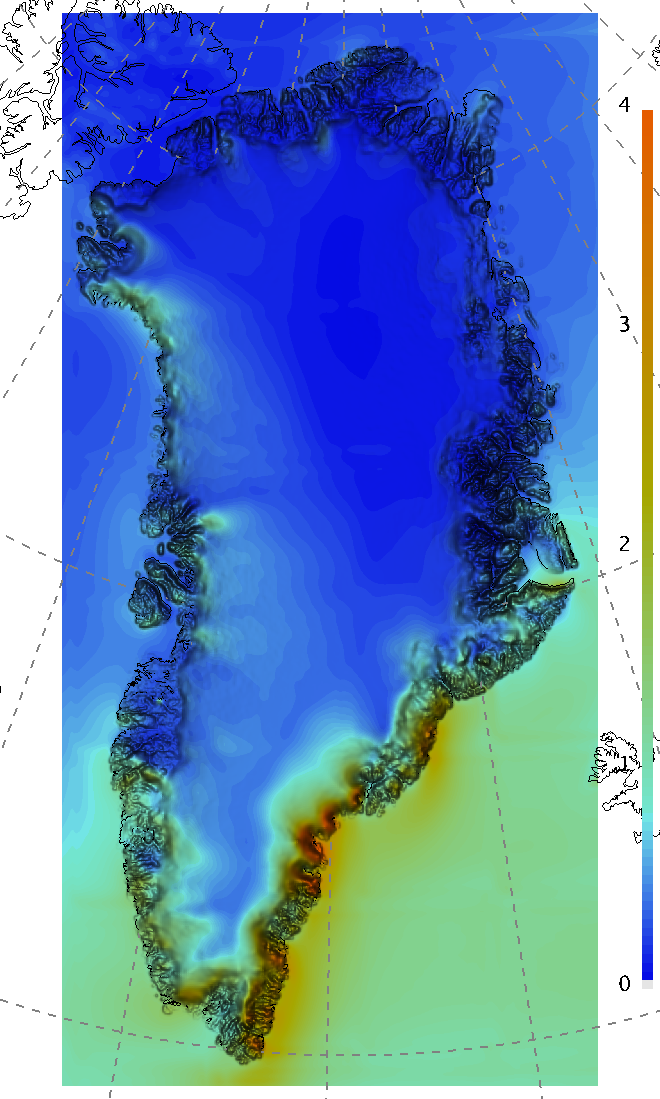
\includegraphics[width=2.0in,keepaspectratio=true]{sr-greenland-prcp}}
\caption{The input present-day ice thickness (left; m), bedrock elevation (center; m), and present-day precipitation (right; m $\text{a}^{-1}$ ice equivalent) for SeaRISE-Greenland.}
\label{fig:sr-input}
\end{figure}


\subsection{Run PISM}   \label{subsect:runscript}  We are ready to run PISM, but, like many Unix programs, PISM allows \emph{a lot} of command-line options.  Furthermore there are configuration parameters that get read from a file (\mbox{\texttt{lib/pism/pism_config.nc}}).  Because PISM handles many different ice sheet, shelf, and glacier configurations, the list of user-configurable flags and parameters is quite long.\footnote{For a complete list see \url{\PISMBROWSERURL}.}  These many options and parameters imply that one should often build a \emph{script} to run PISM with the correct options.  We have done this for \mbox{SeaRISE-Greenland}.

Modeling ice sheets can be done by integrating paleo-climatic and long-time-scale information to build a model for the present state of the ice sheet, so our main script is called ``\texttt{spinup.sh}''.  The spin-up stage is the one which generally requires the most processor-hours, compared to a follow-on ``forecast'' stage.  To \emph{see} what spin-up entails, do this:
\begin{verbatim}
$ PISM_DO=echo
$ ./spinup.sh
\end{verbatim}
Setting the environment variable \texttt{PISM_DO} in this way tells \texttt{spinup.sh} just to print out the commands it is about to run, not do them.  Note that ``\texttt{mpiexec -n 2 pismr}'' appears in the PISM runs done by \texttt{spinup.sh}.  This means that the PISM executable \texttt{pismr} is run in parallel on two processes (e.g.~cores).  The executable name ``\texttt{pismr}'' stands for the standard ``run'' mode of PISM, in contrast to other, specialized modes described later.

For the rest of this example, we assume you have a workstation with 8 cores, but this will all work with 1 to 500 processes, with nearly-proportional scaling in speed.

The script \texttt{spinup.sh} starts by ``bootstrapping.''  This term describes the creation, by heuristics and simplified models, of the kind of full initial conditions needed for the evolving, time-dependent model.  Concretely, the first 100 model year run with 8 processes will look like this (\emph{but there is no need to type here!}):
\small
\begin{verbatim}
mpiexec -n 8 pismr -ocean_kill -e 3 -skip 10 -boot_file pism_Greenland_5km_v1.1.nc \
  -Mx 76 -My 141 -Lz 4000 -Lbz 2000 -Mz 51 -Mbz 21 \
  -atmosphere searise_greenland -surface pdd -pdd_fausto -y 100 -o g20km_pre100.nc
\end{verbatim}
\normalsize
The options describe a $76\times 141$ point grid in the horizontal, which gives 20 km grid spacing in both directions.  There are also important choices about the vertical extent and resolution of the computational grid; more on those later. 

Now, instead of typing-in the above PISM command with all its options, get the run going by resetting the environment variable \texttt{PISM_DO} to empty, and running the script:
\begin{verbatim}
$ export PISM_DO=
$ ./spinup.sh 8 >> out.spin20km &
\end{verbatim}
\noindent Because we have re-directed the text output, PISM will show what it is doing in the text file \texttt{out.spin20km} as it runs in the background.  Using the GNU tool \texttt{less}\index{less, a GNU tool} is a good way to watch such a growing text file.  Reasonably quickly--- within a minute--- the run will produce the early flow result in \texttt{g20km_pre100.nc}.

Soon after that some climatic boundary conditions sample results will appear: \texttt{g20km_climate-500a.nc}, \texttt{g20km_climate-500a.nc}.  Such output from executable \texttt{pclimate} is effectively a movie of the stored and modeled climatic inputs to our ice dynamics model, including the results from surface models like the above-mentioned PDD model for surface mass balance.  This is a convenient way to, early in the modeling process, look at the critical surface mass balance and surface temperature inputs to the ice dynamics.

\subsection{Spin-Up}  \label{subsect:spinupsketch}  The next paragraphs describe what happens and what files are produced by the run which is underway.  We believe that the modeling choices represented here are reasonable, but there is certainly no claim that this is the ``only way to do it''.  The user is encouraged to experiment\dots that is the point of a model.

After the completion of the first 100 model year run (\texttt{g20km_pre100.nc}), we then work to generate a more-credible enthalpy field in which the modeled ice internal energy, its temperature, its softness, its flow velocity, its stored basal water, and its basal melt rate are all in better balance with the ice sheet geometry.  In particular the upper and lower surfaces of this modeled ice are held fixed at this stage.  The upper surface is held fixed by the option \texttt{-no_mass}, while the lower surface is held fixed in the sense that we do not yet apply a bed deformation model.  The resulting enthalpy field is in approximate equilibrium with a velocity field for which the surface kinematical equation \cite{Fowler} is unfortunately \emph{not} satisfied.  Also there is no sliding at this stage because good sliding requires good basal strength which requires good basal melt rates in PISM.

We sometimes call this early stage ``pre-spin-up'', a stage which follows on ``bootstrapping'' and comes before ``actual spin-up'' which uses the paleo-climatic data.  This ``pre-spin-up'' stage goes for 50,000 model years and yields the file \texttt{g20km_steady.nc} at the end.  Along the way the file \texttt{ex_g20km_steady.nc} is updated at every 500 model years, and it can be used to evaluate the degree to which we have reached a thermomechanically-coupled steady state.


\begin{figure}[ht]
\centering
%  temppabase from last time in ex_g10km_steady.nc and driving stress taud from g10km_SIA.nc
\mbox{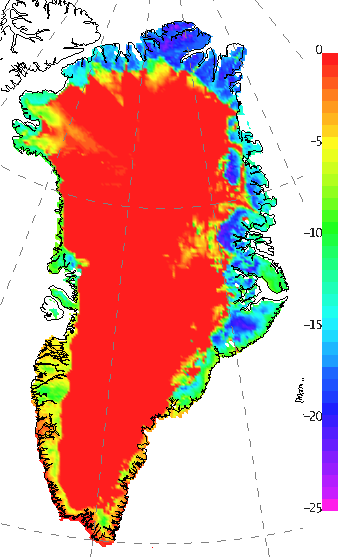
\includegraphics[width=2.0in,keepaspectratio=true]{temppabase}
  \qquad 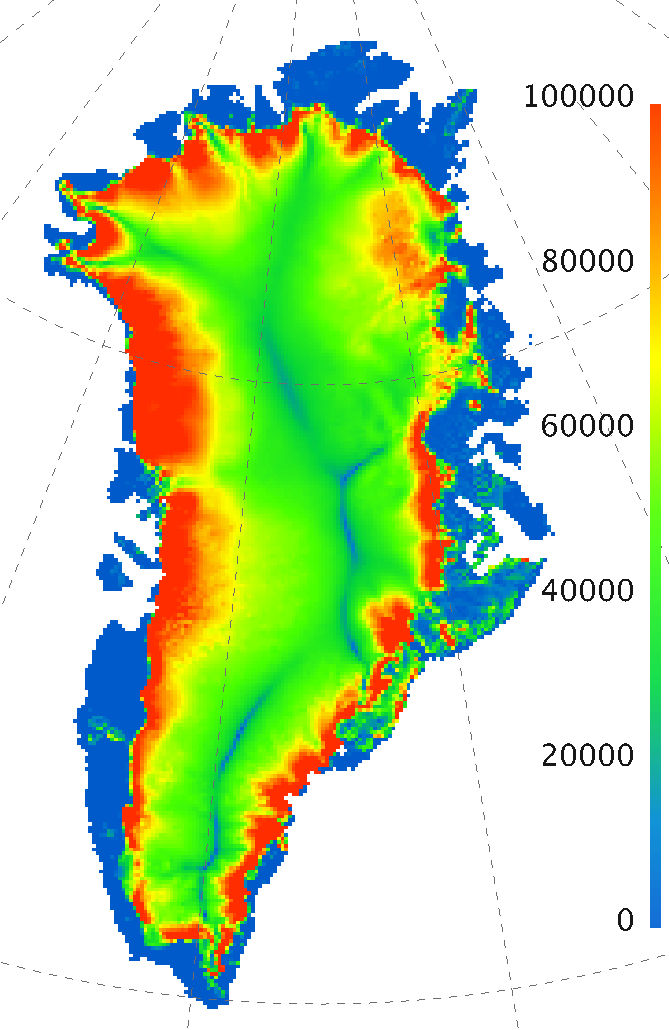
\includegraphics[width=2.1in,keepaspectratio=true]{taud}}
\caption{A look at the model state at the beginning of paleo-climate-modeling ice sheet spin-up.  Left: pressure-adjusted basal temperature ($\phantom{|}^\circ$C).  Right: driving stress $\rho g H |\grad h|$ (Pa).}
\label{fig:sr-spinstart}
\end{figure}

The resulting model state in \texttt{g20km_steady.nc} is our model for the state of the Greenland ice sheet at the beginning of the paleo-climate record provided in the SeaRISE data set, namely 125,000 B.P.  There is, obviously, great uncertainty in this model for the distant past of the Greenland ice sheet.  Two views of the 20\,km model grid version of this state are in Figure \ref{fig:sr-spinstart}.

\begin{figure}[ht]
\centering
%  thk, cbase, csurf from g10km_0.nc
\mbox{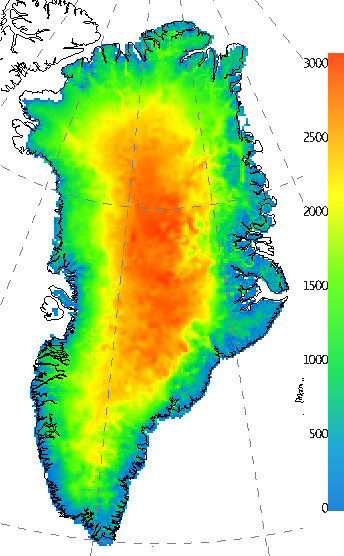
\includegraphics[width=2.in,keepaspectratio=true]{thk}
  \qquad 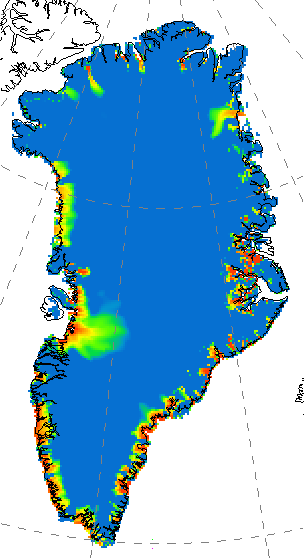
\includegraphics[width=2.in,keepaspectratio=true]{cbase}
  \qquad 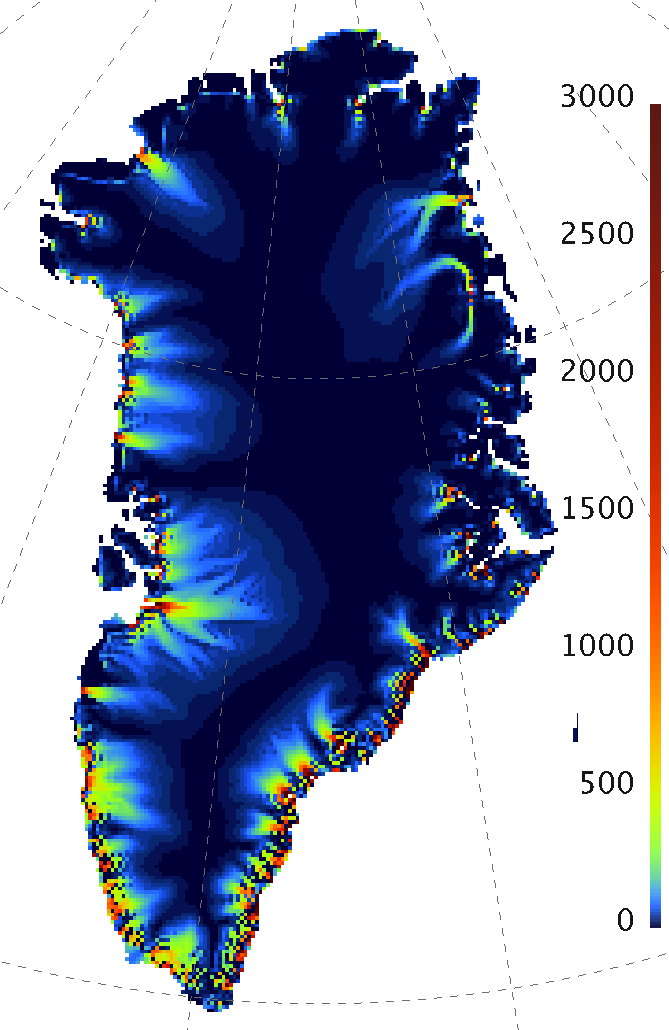
\includegraphics[width=2.in,keepaspectratio=true]{csurf}}
\caption{Model for the present-day Greenland ice sheet, based on spin-up over 125,000 model years using paleo-climate forcing.  Left: ice thickness (m).  Center: basal sliding velocity (m/a).  Right: surface velocity (m/a).}
\label{fig:sr-spindone-map}
\end{figure}


The actual paleo-climate-driven spin-up starts from model state \texttt{g20km_steady.nc}.  We turn on three new mechanisms, climatic forcing, bed deformation, and improved stress balance.  There are two forms of climatic forcing. First, temperature offsets from GRIP core data which affect the snow temperature and thus the surface mass balance, so in warm periods there is more marginal ablation.  Additionally, sea levels from the SPECMAP cores affects which part of the ice are floating. Finally, we turn on the bed deformation model. On the other hand, there is a more complete ice dynamics model with sliding controlled by a membrane stress balance.  Namely, the SIA+SSA hybrid model.

The run now goes from the SeaRISE-Greenland-chosen start time of -125,000 years to -10,000 years.  In this period, diagnostic outputs are written into \texttt{ex_g20km_m10ka.nc} at every 500 model years, and scalar time series including total ice volume are written into \texttt{ts_g20km_m10ka.nc} at every model year.  At the end of this period we get the model state file \texttt{g20km_m10ka.nc}. Unless you run \texttt{./spinup N 2}, the following run continues on the same grid from -10,000 years to present day, producing \texttt{g20km_0.nc}.

The spun-up state \texttt{g20km_0.nc} is intended to be a model for the Greenland ice sheet at the present day, and thus a basis on which to explore future ice sheet behavior.  Figure \ref{fig:sr-spindone-map} shows some fields from the 20\,km model grid version of this present-day state.  The ice sheet thickness and surface velocity should be compared to present-day observations \cite{BKAJS}, and parameter dependences in the spin-up process should be explored.

Over the course of the spin-up we have saved the modeled ice volume in ``time-series'' NetCDF files.  This important model output can be viewed by
\begin{verbatim}
$ ncview ts_g20km_m20ka.nc ts_g20km_0.nc
\end{verbatim}
\noindent Figure \ref{fig:sr-spindone-ivolboth} shows this ice volume time series for the whole spin-up.  We see the modeled volatility of ice volume in the late ``Eemian'' period, between -120,000 and -115,000 BPE in the SeaRISE version of the GRIP temperature data.

\begin{figure}[ht]
\centering
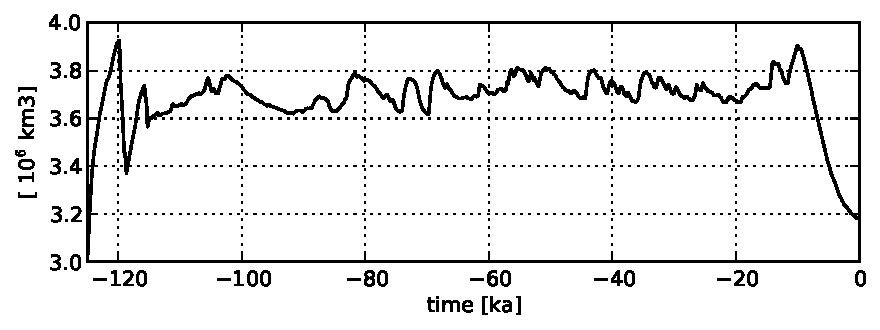
\includegraphics[width=5.6in,keepaspectratio=true]{ivol}
\caption{Time series of modeled ice sheet volume on 20km grid.}
\label{fig:sr-spindone-ivolboth}
\end{figure}

The total run time for the complete 20\,km spin-up, which models 125,000 model years with ``full physics'' of the polythermal SIA+SSA hybrid type (section \ref{sect:dynamics}) uses about 60 processor-hours.  If done without membrane stresses (SIA only) this computational time is reduced.  The polythermal (vs ``cold'') physics choice has no significant performance disadvantage.


\subsection{Going forward}  \label{subsect:forecastcaution}  In the same \verb|examples/searise-greenland| directory is a script \verb|forecast.sh|.  (If your spun-up state is called \texttt{g20km_0.nc}, then run  \verb|./forecast.sh 8 g20km_0.nc|, assuming you have 8 cores.  It does two runs for 100 years into the future, initializing from the modeled present-day state. The first run is a ``control''  run assuming steady climate for the entire 100 year period. The second runs uses AR4 climate forcing. Please run it, play with it, and modify it, but remember that it is merely a demonstration.

Because ice sheets, and ice sheet models, have a ``memory'' of past climates, whether real or modeled, the results strongly depend on the nature of the spin-up process which preceded this ``forecast'' run.  Therefore, as already noted, it is critical to evaluate the quality of the spunup state, for example using present-day observations of surface velocity \cite{BKAJS}, and other observations including ice temperature in ice bore-holes.  Critical thinking about a broad range of modeling hypotheses is prerequisite to building models of future behavior.  Naive or casual use of PISM to generate ice sheet predictions is \emph{not} recommended!


\subsection{Handling NetCDF files}\label{subsect:nctoolsintro}  At a superficial level, PISM is just a program which takes one or more NetCDF files as input, does some computation, and produces one or more NetCDF files as output.  As a result, the user needs tools to extract some meaning from the NetCDF output files and also, in the general case, more tools to create NetCDF files for input to PISM.\footnote{Regarding the creation of input files, see the section \ref{sec:bootstrapping-format} and table \ref{tab:modelhierarchy} for ideas about the data necessary for modeling.}

The most basic tools for converting NetCDF files to and from a standard text representation are called \texttt{ncdump} and \texttt{ncgen}.  A glance at Unix \texttt{man} pages for these tools might be wise at this time.

We most-regularly use \texttt{ncview} to look at NetCDF files.  Table \ref{tab:NetCDFview} lists NetCDF tools that can be useful for visualizing and post-processing PISM output files, as well as for preparing input data.  We find \texttt{ncview}, NCO, IDV and PyNGL especially useful.

\newcommand{\netcdftool}[1]{#1\index{NetCDF!tools!#1}}
\begin{table}[ht]
\centering
\caption{Some tools for viewing and modifying NetCDF files.}\label{tab:NetCDFview} 
\small
\begin{tabular}{llp{0.4\linewidth}}
  \\\toprule
  \textbf{Tool} & \textbf{Site} & \textbf{Function}\\ \midrule
\netcdftool{\texttt{ncdump}} & \emph{included with any NetCDF distribution} & dump binary NetCDF as \texttt{.cdl} (text) file \\
\netcdftool{\texttt{ncgen}} & \emph{included with any NetCDF distribution} & convert \texttt{.cdl} file to binary NetCDF \\
\netcdftool{\texttt{ncview}} & \href{http://meteora.ucsd.edu/~pierce/ncview_home_page.html}{\texttt{meteora.ucsd.edu/$\sim$pierce}} & quick graphical view \\
\netcdftool{IDV} & \href{http://www.unidata.ucar.edu/software/idv/}{\t{www.unidata.ucar.edu/software/idv/}} & more complete visualization \\
%\netcdftool{Paraview} & \href{http://www.paraview.org}{\t{www.paraview.org}} & powerful open-source parallel visualization \\
\netcdftool{NCL} &  \href{http://www.ncl.ucar.edu}{\t{www.ncl.ucar.edu}} & NCAR Command Language\\
\netcdftool{PyNGL} &  \href{http://www.pyngl.ucar.edu}{\t{www.pyngl.ucar.edu}} & Python version of NCL\\
%\netcdftool{VisIt} & \href{http://visit.llnl.gov}{\t{visit.llnl.gov}} & advanced parallel visualization \\
\netcdftool{NCO}\index{NCO (NetCDF Operators)} & \href{http://nco.sourceforge.net/}{\t{nco.sourceforge.net/}} & NetCDF Operators; command-line tools\\
\netcdftool{CDO} & \href{http://code.zmaw.de/projects/cdo}{\texttt{www.mpimet.mpg.de/fileadmin/software/cdo/}} & Climate Data Operators; more command-line tools, including conservative re-mapping \\
 & \href{http://www.unidata.ucar.edu/software/netcdf/}{\texttt{www.unidata.ucar.edu/software/netcdf/}} & root for NetCDF information
\\\bottomrule
\end{tabular}
\normalsize
\end{table}


%%% Local Variables: 
%%% mode: latex
%%% TeX-master: "manual"
%%% End: 


% LocalWords:  metadata SPECMAP paleo html IDV
